\documentclass[11pt,a4paper]{article}
\usepackage[utf8]{inputenc}
\usepackage[T1]{fontenc}
\usepackage{lmodern}
\usepackage[margin=1.85cm]{geometry}
\usepackage{amsmath,amssymb,amsthm}
\usepackage{booktabs}
\usepackage{array}
\usepackage{graphicx}
\usepackage{xcolor}
\usepackage{hyperref}
\emergencystretch=2.2em
\sloppy

\definecolor{linkblue}{HTML}{1D4ED8}
\hypersetup{
    colorlinks=true,
    linkcolor=linkblue,
    citecolor=linkblue,
    urlcolor=linkblue,
    pdftitle={Kodama-Hayward Galactic Acceleration Trough vs. DES Year 6 Dynamical Dark Energy: Background-Dependence Theorem, Direct Multi-Probe BAO/CMB/Supernova Tests, and Void-Volume-Weighted Optical Models},
    pdfauthor={Jozsef Olcsak (ORCID: 0009-0003-7311-6522)}
}

\newtheorem{theorem}{Theorem}
\newtheorem{proposition}{Proposition}
\newtheorem{corollary}{Corollary}
\theoremstyle{definition}
\newtheorem{hypothesis}{Hypothesis}

\title{\textbf{\Large Kodama--Hayward Galactic Acceleration Trough vs.\ \texttt{DES} Year~6 Dynamical Dark Energy}\\[0.35em]
\large Background-Dependence Theorem, Direct \texttt{Pantheon++DESI BAO+CMB} Likelihood Tests, and Void-Volume-Weighted Optical Models}

\author{\textbf{Jozsef Olcsak}\\[0.2em]
{\small Independent Researcher $\cdot$ ORCID: \href{https://orcid.org/0009-0003-7311-6522}{0009-0003-7311-6522}}\\[0.2em]
{\small Permanent Code \& Data Archives: \href{https://doi.org/10.5281/zenodo.24354218}{doi:10.5281/zenodo.24354218} $\cdot$ \href{https://doi.org/10.5281/zenodo.24305895}{doi:10.5281/zenodo.24305895}}}
\date{19 November 2026 (Revised Referee Edition v6.0)}

\begin{document}
\maketitle

\begin{abstract}
\noindent Combining the full 6-year Dark Energy Survey dataset (\texttt{DES-SN5YR}, BAO, and $3\times 2\mathrm{pt}$ weak lensing/clustering) with primary CMB constraints yields a $\sim 3.0\sigma$ preference for dynamical dark energy ($w_0 = -0.82 \pm 0.05$, $w_a = -0.63^{+0.21}_{-0.18}$; \texttt{DES} Collaboration 2026, \texttt{arXiv:2605.27221}; cf.\ \texttt{DESI} DR2, \texttt{arXiv:2503.14738}), whereas replacing \texttt{DES-SN5YR} with the $1,580$-supernova \texttt{Pantheon+} Hubble-flow compilation shifts the joint \texttt{Pantheon++DESI BAO+CC+CMB+BBN} ($N=1,610$) free-CPL optimum to $(w_0, w_a) = (-0.8895 \pm 0.0597,\; -0.2250 \pm 0.2686)$ ($\rho = -0.8860$) at information-criterion parity with $\Lambda$CDM ($\Delta\chi^2 = -6.53$, $\Delta\mathrm{AIC} = -2.53$, $\Delta\mathrm{BIC} = +8.24$; Efstathiou, \textit{MNRAS} \textbf{538}, 875, 2025). Concurrently, Lane, Seifert, Ridden-Harper, and Wiltshire (\textit{MNRAS} \textbf{536}, 1752, 2025; \textit{MNRAS Lett.} \textbf{537}, L55, 2025) showed that faster proper clocks inside expanding cosmic voids ($\mathrm{d}\tau/\mathrm{d}t > 1$) cause single-clock FLRW fits to infer an apparent $w_0^{\mathrm{app}} > -1$ without a dark-energy fluid, though unweighted pure Timescape on standard SALT2 \texttt{Pantheon+} yields $\chi^2_{\mathrm{SN}} = 1403.83$ ($\Delta\chi^2 = +16.50$ vs.\ $\Lambda$CDM) and leaves galactic rotation curves unmodeled. Here we establish four results with strict separation between proven theorems and phenomenological models: (1) \textbf{Theorem~\ref{thm:kh-background} (\texttt{PROVEN} \& tested with asymptotic-flat MOND/RAR kernels):} For apparent-horizon Kodama--Hayward scaling $a_0(z) \propto cH(z)|1-q(z)|$, coincidence between the galactic trough $z_{\mathrm{dip}}$ and acceleration onset $q(z_{\mathrm{acc}})=0$ holds iff $3w(1+w) = \mathrm{d}w/\mathrm{d}\ln a$ at $z_{\mathrm{acc}}$; a homogeneous \texttt{DES} CPL fluid erases the $w_{\mathrm{hor}}=-1$ trough ($0.938550 \to 1.142720$ at $z=0.6316$), degrading the post-trough ($0.787 \le z \le 1.03$) fit across $43$ \texttt{JWST/HST} disk galaxies (Mancera Pi\~na \textit{et al.}\ 2025) under both Milgrom's standard MOND ($\chi^2 = 107.53 \to 121.65$, $\Delta\chi^2 = +14.12$ raw / $+5.65$ rescaled at canonical $a_0(0)=1.20\times 10^{-10}\;\mathrm{m\,s^{-2}}$; or $95.93 \to 102.49$ at $a_0^{\mathrm{KH}}(0)=0.9015\times 10^{-10}\;\mathrm{m\,s^{-2}}$) and McGaugh's RAR ($186.55 \to 217.44$, $\Delta\chi^2 = +30.89$ / $+7.12$ rescaled), while we formally retract deep-MOND RAR equivalence for the companion logarithmic kernel ($v \propto r^{-1/2}\ln r \to 0$ as $r\to\infty$); (2) \textbf{Theorem~\ref{thm:forward-nogo} (\texttt{PROVEN}):} Following Kantowski (1969), Dyer \& Roeder (1972, 1973), and Weinberg (1976), single-clock beam de-focusing leaves $D_A''(0)$ invariant because $D_A(0)=0$, forcing $w_0^{\mathrm{app}}(0) \equiv -1$, while weak-field QUMOND void potentials yield $|\Delta w_0^{\mathrm{app}}| < 10^{-3}$; (3) \textbf{Proposition~\ref{prop:void-fraction} (\texttt{CONDITIONAL} Calibration~\ref{hyp:H1}):} Matching $q_{\mathrm{wall}}(f_{\mathrm{acc}}) = 0$ ($f_{\mathrm{acc}} = 0.586708$) to $z_{\mathrm{acc}}^{\mathrm{hor}} = 0.631556$ calibrates $f_{v,0} = 0.7234$ ($\mathrm{d}f_{v,0}/\mathrm{d}z_{\mathrm{acc}} \approx 0.141$); and (4) \textbf{Proposition~\ref{prop:ocsr-void-clock} (\texttt{PHENOMENOLOGICAL} Direct \texttt{SN+DESI BAO+CMB} Fit \& $\alpha$-Profile):} On \texttt{Pantheon+} alone, split-beam models are \emph{statistically equivalent} to $\Lambda$CDM ($\Delta\chi^2_{\mathrm{SN}} = -0.74$ to $-1.21$, with $\alpha \in [0,0.43]$ unconstrained due to $\Omega_{m,0}$ degeneracy), and universal constant-weight \textbf{H2a} ($p=0$) is \emph{ruled out} by CMB $\theta_*$ + BAO ($\Delta\chi^2 = +5.56$) because nonlinear voids vanish at recombination ($z_* \simeq 1090$). Weighting the Wiltshire (2009) transit rate by the physical void volume fraction $\alpha_{\mathrm{eff}}(z) = \alpha\,f_v(z)/f_{v,0}$ ($p=1$, vanishing automatically as $z \to z_*$) breaks the $\Omega_{m,0}$ degeneracy across the joint $N=1,610$ \texttt{Pantheon++DESI BAO+CC+CMB $\theta_*$+BBN} dataset: unconstrained profiling yields $\hat{\alpha}_{\mathrm{MLE}} = \mathbf{0.330 \pm 0.139}$ ($\Delta\chi^2 = -6.52$, $\sim 2.55\sigma$ over $\alpha=0$ while excluding pure Timescape $\alpha=1$ at $+11.02$), and fixing the prior hypothesis $\alpha_0 = \frac{5\sqrt{3}}{24} = 0.3608$ ($0.22\sigma$ from $\hat{\alpha}_{\mathrm{MLE}}$, $k=4$, zero extra parameters vs.\ $\Lambda$CDM) yields $\Delta\chi^2 = \mathbf{-6.47}$ ($\Delta\mathrm{AIC} = \Delta\mathrm{BIC} = -6.47$ vs.\ $\Lambda$CDM, $\Delta\mathrm{BIC} = \mathbf{-14.71}$ vs.\ free CPL; $\Delta\chi^2 = \mathbf{-6.57}$ on \texttt{SN+BAO+CMB+BBN} without CC, and $\mathbf{-6.37}$ for \textbf{Forward \texttt{H2-Sachs}}).
\end{abstract}

\section{Introduction: Multi-Probe Supernova, Void-Clock, and Disk-Rotation Tensions}
Observational cosmology currently confronts three interlocking questions across $0.01 \le z \le 1.2$:
\begin{enumerate}
    \item \textbf{\texttt{DES} Year~6 vs.\ \texttt{Pantheon+} Supernovae in Multi-Probe CPL Fits:} In the full 6-year Dark Energy Survey analysis \cite{DES2026DynDE}, \texttt{DES} Y6 probes alone (\texttt{DES-SN5YR} \cite{DESSN5YR2024}, BAO, and $3\times 2\mathrm{pt}$) yield $w_0 = -0.84 \pm 0.10$, $w_a = -0.44^{+0.60}_{-0.55}$ ($2.2\sigma$), \texttt{DES} Y6 + \texttt{DESI} BAO gives $w_0 = -0.84^{+0.06}_{-0.07}$, $w_a = -0.53^{+0.33}_{-0.28}$ ($2.3\sigma$), and combining \texttt{DES} Y6 with primary \texttt{Planck} CMB gives $w_0 = -0.82 \pm 0.05$, $w_a = -0.63^{+0.21}_{-0.18}$ ($\sim 3.0\sigma$; see also \texttt{DESI} DR2 \cite{DESIDR2_2025}). However, Efstathiou \cite{Efstathiou2025SN} identified a $\sim 0.04\;\mathrm{mag}$ low-$z$/high-$z$ cross-calibration offset between \texttt{DES-SN5YR} and \texttt{Pantheon+} \cite{Brout2022}. Replacing \texttt{DES-SN5YR} with the bundled $N=1,580$ non-calibrator \texttt{Pantheon+} Hubble-flow sample in our joint $N=1,610$ likelihood (\texttt{Pantheon+} + $13$ \texttt{DESI} BAO + $15$ Moresco cosmic chronometers + \texttt{Planck} CMB $100\theta_*$ + Cooke BBN $\omega_b$) shifts the free-CPL optimum (\texttt{M1b}) to $(w_0, w_a) = (\mathbf{-0.8895 \pm 0.0597},\; \mathbf{-0.2250 \pm 0.2686})$ (exact $5\times 5$ Hessian marginalization, $\rho = -0.8860$) at statistical parity with $\Lambda$CDM ($\Delta\chi^2 = -6.53$, $\Delta\mathrm{AIC} = -2.53$, $\Delta\mathrm{BIC} = +8.24$, Table~\ref{tab:multiprobe}).
    \item \textbf{\textit{MNRAS} 2025 Inhomogeneous Void-Clock (\emph{Timescape}) Cosmology:} Independently, Lane, Seifert, Ridden-Harper, and Wiltshire \cite{LaneWiltshire2025MNRAS} and Seifert \textit{et al.} \cite{SeifertWiltshire2025MNRAS} showed that when supernova photons traverse a cosmic web partitioned into bound filaments (wall proper time $t_w$) and expanding underdense voids (volume fraction $f_v(z)$, faster clock rate $\bar{\gamma} = \mathrm{d}t/\mathrm{d}t_w = 1 + \frac{1}{2}f_v > 1$), fitting a single-clock flat-FLRW template to $D_L(z)$ yields an \emph{apparent} $w_0^{\mathrm{app}} > -1$, $w_a^{\mathrm{app}} < 0$ without a dark-energy fluid. Yet standalone Timescape \cite{Wiltshire2009PRD,LaneWiltshire2025MNRAS} leaves $f_{v,0}$ as a free parameter, yields $\chi^2_{\mathrm{SN}} = 1403.83$ ($\Delta\chi^2_{\mathrm{SN}} = +16.50$ vs.\ $\Lambda$CDM $1387.33$; best-fit $f_{v,0}=0.8526$ gives $1391.55$) on standard SALT2 \texttt{Pantheon+} covariances, and provides no law for galactic rotation curves.
    \item \textbf{Apparent-Horizon Kodama--Hayward Scaling $a_0(z)$ and Asymptotic-Flat Rotation Curves:} On a non-stationary flat FLRW background, the Kodama--Hayward surface gravity of the apparent horizon $r_{\mathrm{AH}} = c/H(z)$ is $|\kappa_{\mathrm{KH}}(z)| = \frac{1}{2}cH(z)|1 - q(z)|$ (Cai--Kim convention). Coupling galactic acceleration linearly to $|\kappa_{\mathrm{KH}}(z)|$ yields
    \begin{equation}
        a_0(z) = a_0(0)\,\frac{H(z)\,\bigl|1 - q(z)\bigr|}{H_0\,\bigl|1 - q_0\bigr|}, \qquad a_0^{\mathrm{KH}}(z) := \frac{1}{2}\alpha_0\,\bigl|\kappa_{\mathrm{KH}}(z)\bigr| = \frac{\alpha_0}{4}\,c H(z)\,\bigl|1 - q(z)\bigr|,
        \label{eq:a0-kh-universal}
    \end{equation}
    where we test both the empirical canonical MOND/RAR normalization $a_{0,\mathrm{MOND}}(0) = 1.20\times 10^{-10}\;\mathrm{m\,s^{-2}}$ \cite{Milgrom1983,McGaugh2016} and the pre-fixed companion-model coupling hypothesis $\alpha_0 = \frac{5\sqrt{3}}{24} \approx 0.360844$ ($a_0^{\mathrm{KH}}(0) = 0.9015\times 10^{-10}\;\mathrm{m\,s^{-2}}$ at Planck $\Omega_{m,0}=0.3153$, $H_0=67.36\;\mathrm{km\,s^{-1}\,Mpc^{-1}}$) \cite{TauCoreZenodo2026}, auditing $\alpha$ explicitly against an unconstrained empirical profile over $\alpha \in [0,1]$ so no external algebraic ansatz need be assumed.
\end{enumerate}

\paragraph{Retraction of Deep-MOND RAR Equivalence for the Companion Logarithmic Kernel.} An earlier draft invoked the companion finite-disk logarithmic velocity kernel $v_{\mathrm{log}}(r) = v_{\mathrm{bar}}(r)\bigl[1 + \alpha_0(1 - e^{-\mu u})\ln(1+u)\bigr]$ ($u = a_0/a_N$) and stated that it corresponded directly to McGaugh's RAR \cite{McGaugh2016}. \emph{We formally retract that deep-MOND equivalence claim:} around a point mass as $r \to \infty$ ($u \propto r^2 \to \infty$), $v_{\mathrm{log}}(r) \propto r^{-1/2}\ln r \to 0$, so it possesses neither an asymptotically flat rotation speed $v_\infty = (GM_b a_0)^{1/4}$ nor a strict asymptotic BTFR ($g_{\mathrm{obs}}/g_{\mathrm{bar}} = [1.43, 3.14, 6.57, 11.49]$ vs.\ McGaugh RAR $[1.58, 3.69, 10.51, 32.13]$ at $g_{\mathrm{bar}}/a_{0,\mathrm{MOND}} = [1, 10^{-1}, 10^{-2}, 10^{-3}]$). Accordingly, Theorem~\ref{thm:kh-background} is tested here primarily using **true asymptotic-flat MOND and RAR interpolation functions** with zero auxiliary screening parameter $\mu$.

\section{Theorem 1: Background Dependence of $a_0(z)$ and Asymptotic-Flat MOND/RAR Audit on 43 Disks}

\begin{theorem}[Coincidence-Breaking Identity under General $w(z)$ and Asymptotic-Flat 43-Disk Test]
\label{thm:kh-background}
Let a spatially flat FLRW background contain pressureless matter $\Omega_{m,0} \in (0,1)$ and smooth dark energy $\Omega_{\mathrm{DE},0} = 1 - \Omega_{m,0}$ with equation of state $w(a)$ and density ratio $W(a) := \rho_{\mathrm{DE}}(a)/\rho_{\mathrm{DE},0} = \exp\bigl[-3\int_a^1 (1+w(\tilde{a}))\,\mathrm{d}\ln\tilde{a}\bigr]$. Then:
\begin{enumerate}
    \item \textbf{Monotonic Activation No-Go:} Since $1 + w(a) = -\frac{1}{3}\frac{\mathrm{d}\ln W(a)}{\mathrm{d}\ln a}$, no monotonic $W(a)$ can cross $w = -1$.
    \item \textbf{Equivalence-Breaking Identity and Exact Slope at $q(z_{\mathrm{acc}}) = 0$:} For general $w(z)$, $\frac{1 - q(z)}{2} - \bigl(1 - \frac{3}{4}\Omega_m(z)\bigr) = -\frac{3}{4}\bigl(1 + w(z)\bigr)\Omega_{\mathrm{DE}}(z)$, and the logarithmic derivative of $a_0(z) \propto H(z)|1-q(z)|$~\eqref{eq:a0-kh-universal} at $q(z_{\mathrm{acc}}) = 0$ ($\Omega_{\mathrm{DE}}(z_{\mathrm{acc}}) = -\frac{1}{3w(z_{\mathrm{acc}})}$) is
    \begin{equation}
        \left.\frac{1}{a_0}\frac{\mathrm{d}a_0}{\mathrm{d}\ln a}\right|_{q=0} = \left.\frac{1}{H}\frac{\mathrm{d}\bigl[H(1-q)\bigr]}{\mathrm{d}\ln a}\right|_{q=0} = -\frac{3}{2}\bigl(1 + w(a_{\mathrm{acc}})\bigr) + \frac{1}{2w(a_{\mathrm{acc}})}\left.\frac{\mathrm{d}w}{\mathrm{d}\ln a}\right|_{a_{\mathrm{acc}}}.
        \label{eq:coincidence-breaking}
    \end{equation}
    Hence $z_{\mathrm{dip}} = z_{\mathrm{acc}}$ holds if and only if $3w(1+w) = \frac{\mathrm{d}w}{\mathrm{d}\ln a}$ at $z_{\mathrm{acc}}$ (uniquely $w = -1$ for constant $w \neq 0$, giving a $-6.15\%$ trough $a_0(z_{\mathrm{dip}})/a_0(0) = 0.938550$ at $z_{\mathrm{dip}} = 0.631556$).
    \item \textbf{Erasure of the Trough and Post-Trough Test with Asymptotic-Flat MOND/RAR Kernels on 43 \texttt{JWST/HST} Disks:} On the homogeneous \texttt{DES} Y6 + \texttt{CMB} CPL mean ($w_0 = -0.82$, $w_a = -0.63$, $\Omega_{m,0} = 0.3153$), $\bigl[a_0(0.6316)/a_0(0)\bigr]_{\mathrm{DES\text{-}CPL}} = \mathbf{1.142720}$ ($+21.75\%$, erasing the $z > 0$ minimum in $99.725\%$ of draws). Evaluating the $43$ \texttt{JWST/HST} disk galaxies of Mancera Pi\~na \textit{et al.} \cite{ManceraPina2025} ($0.787 \le z \le 1.03$, post-trough $r_{\mathrm{eval}} = 2R_{\mathrm{eff}}$ with Tacconi+20 gas scaling) using standard interpolation laws that satisfy exact $r \to \infty$ flatness $v_\infty = (GM_b a_0(z))^{1/4}$:
    \begin{itemize}
        \item \textbf{Standard Milgrom (1983) MOND $\mu_{\mathrm{std}}(y) = y/\sqrt{1+y^2}$ \cite{Milgrom1983} at canonical $a_0(0) = 1.20\times 10^{-10}\;\mathrm{m\,s^{-2}}$:} $w_{\mathrm{hor}} = -1$ Kodama--Hayward gives $\chi^2 = \mathbf{107.53}$ ($\chi^2/\mathrm{dof} = \mathbf{2.501}$) vs.\ $\chi^2 = \mathbf{121.65}$ for $z=0$-anchored \texttt{DES}-CPL ($\Delta\chi^2 = \mathbf{+14.12}$ raw / $\mathbf{+5.65}$ rescaled by $\chi^2/\mathrm{dof}$), $\chi^2 = \mathbf{111.45}$ unanchored ($\Delta\chi^2 = +3.92$ raw, while dropping $a_0(0)$ by $-12.11\%$), and $\chi^2 = \mathbf{169.44}$ for monotonic $a_0 \propto H(z)$ ($\Delta\chi^2 = \mathbf{+61.91}$). (At $a_0^{\mathrm{KH}}(0) = 0.9015\times 10^{-10}\;\mathrm{m\,s^{-2}}$, $\chi^2 = \mathbf{95.93}$, $\chi^2/\mathrm{dof} = \mathbf{2.231}$, vs.\ $102.49$ anchored and $131.05$ monotonic $H(z)$.)
        \item \textbf{McGaugh \textit{et al.}\ (2016) Empirical RAR $\nu_{\mathrm{RAR}}(y) = (1 - e^{-\sqrt{y}})^{-1}$ \cite{McGaugh2016} at $a_0(0) = 1.20\times 10^{-10}\;\mathrm{m\,s^{-2}}$:} $w_{\mathrm{hor}} = -1$ gives $\chi^2 = \mathbf{186.55}$ vs.\ $\mathbf{217.44}$ for anchored \texttt{DES}-CPL ($\Delta\chi^2 = \mathbf{+30.89}$ raw / $\mathbf{+7.12}$ rescaled), $\mathbf{195.89}$ unanchored, and $\mathbf{297.76}$ for monotonic $a_0 \propto H(z)$ ($\Delta\chi^2 = \mathbf{+111.21}$; at $a_0^{\mathrm{KH}}(0)$, $150.75$ vs.\ $173.29$, $\Delta\chi^2 = +22.54$ / $+6.43$ rescaled).
    \end{itemize}
\end{enumerate}
\end{theorem}

\begin{proof}
Using $\frac{\mathrm{d}\ln H}{\mathrm{d}\ln a} = -(1+q)$, $1-q = \frac{1}{2} - \frac{3}{2}w\Omega_{\mathrm{DE}}$, and $\frac{\mathrm{d}\Omega_{\mathrm{DE}}}{\mathrm{d}\ln a} = -3w(1-\Omega_{\mathrm{DE}})\Omega_{\mathrm{DE}}$ at $q = 0 \iff \Omega_{\mathrm{DE}} = -\frac{1}{3w}$ yields Eq.~\eqref{eq:coincidence-breaking}. At $(-0.82,-0.63,0.3153)$ and $z = 0.6315565$, $E(z) = 1.450613$, $q(z) = -0.057302$, and $1 - q(0) = 1.342181$, giving $\frac{1.450613\times 1.057302}{1.342181} = 1.142720$. Verified in \texttt{verify\_C5} and \texttt{verify\_C9}. \qed
\end{proof}

\section{Theorem 2: Single-Clock Dyer--Roeder and Weak-Field QUMOND Optical No-Go}

\begin{theorem}[Classical Single-Clock $O(z^2)$ Focusing Invariance and Weak-Field Void Bound]
\label{thm:forward-nogo}
Contracting any metric-trace-extended gravitational field equation ($G_{\mu\nu} + \Lambda_{\mathrm{eff}}g_{\mu\nu} - \frac{1}{2}V_{\mathrm{QUMOND}}(y)g_{\mu\nu} = \frac{8\pi G}{c^4}T^{\mathrm{eff}}_{\mu\nu}$) with a null wavevector $k^\mu$ ($g_{\mu\nu}k^\mu k^\nu = 0$) annihilates all $g_{\mu\nu}$-proportional terms. On a single-clock $w_{\mathrm{hor}} = -1$ FLRW background ($E_{\mathrm{ray}}(z) = E_{\mathrm{hor}}(z)$):
\begin{enumerate}
    \item \textbf{Exact $w_0^{\mathrm{app}}(z \to 0) \equiv -1$ Invariance \cite{Kantowski1969,DyerRoeder1973,Weinberg1976}:} In the forward Dyer--Roeder / Sachs equation with arbitrary smooth focusing fraction $\alpha_{\mathrm{beam}}(z)$, $\frac{\mathrm{d}}{\mathrm{d}z}\bigl[(1+z)^2 E_{\mathrm{hor}}(z)\frac{\mathrm{d}D_A}{\mathrm{d}z}\bigr] + \frac{3}{2}\Omega_{m,0}\alpha_{\mathrm{beam}}(z)\frac{(1+z)^3}{E_{\mathrm{hor}}(z)}D_A(z) = 0$ ($D_A(0)=0$, $D_A'(0)=c/H_0$), the Ricci focusing term vanishes at $z=0$ because $D_A(0)=0$, leaving $D_A(z)$ independent of $\alpha_{\mathrm{beam}}(z)$ through $\mathcal{O}(z^2)$ \cite{Kantowski1969,DyerRoeder1973,Weinberg1976}: $\frac{H_0}{c}D_A''(0) = -(2 + \frac{3}{2}\Omega_{m,0})$, hence $w_0^{\mathrm{app}}(z \to 0) \equiv -1$ identically ($\alpha_{\mathrm{beam}} = 1 - \alpha_0$ enters at $\mathcal{O}(z^3)$ and gives CPL $(-0.8173, -1.5886)$, $\chi^2_{\mathrm{SN}} = 1394.31$).
    \item \textbf{Order-of-Magnitude Weak-Field QUMOND Void Bound:} For cosmic megavoids ($R_v \sim 35\,h^{-1}\;\mathrm{Mpc}$, $\delta_v \approx -0.8$), $g_{N,v}/a_{0,\mathrm{MOND}} = 0.00535$ gives simple-QUMOND boost $\nu_{\mathrm{QUMOND}} = 14.18$, keeping $|\Phi|/c^2 \sim 5\times 10^{-4} \ll 1$ and $|\Delta w_0^{\mathrm{app}}| < 10^{-3}$. Producing $w_0^{\mathrm{app}}(0) > -1$ thus requires an $\mathcal{O}(1)$ proper-clock differential $\mathrm{d}\tau/\mathrm{d}t > 1$ in $\mathrm{d}z/\mathrm{d}\lambda$.
\end{enumerate}
\end{theorem}

\section{Proposition 1: Conditional Void-Fraction Calibration $f_{v,0} = 72.34\%$ under Hypothesis H1}

\begin{hypothesis}[Horizon--Wall Acceleration Transition Matching --- \textbf{H1}]
\label{hyp:H1}
The redshift at which the dressed wall-frame deceleration parameter $q_{\mathrm{wall}}(f_v)$ crosses zero in the Buchert--Wiltshire tracker coincides with the apparent-horizon inflection redshift $z_{\mathrm{acc}}^{\mathrm{hor}} = (2\Omega_{\Lambda,0}/\Omega_{m,0})^{1/3} - 1$: $z(f_{\mathrm{acc}}) = z_{\mathrm{acc}}^{\mathrm{hor}}$.
\end{hypothesis}

\begin{proposition}[Conditional Algebraic Void-Fraction Calibration and Jacobian Sensitivity]
\label{prop:void-fraction}
In the Buchert--Wiltshire tracker \cite{Wiltshire2009PRD,LaneWiltshire2025MNRAS,SeifertWiltshire2025MNRAS}, $q_{\mathrm{wall}}(f_v) = \frac{8f_v^4 + 31f_v^3 - 51f_v^2 + 4f_v + 8}{16f_v^4 + 8f_v^3 + 33f_v^2 + 8f_v + 16}$ crosses zero at the unique physical root $f_{\mathrm{acc}} = \mathbf{0.58670773}$ ($58.67\%$). Along $1 + z(f_v) = \frac{2+f_v}{2+f_{v,0}}\bigl(\frac{f_{v,0}}{f_v}\bigr)^{2/3}\frac{1-f_v}{1-f_{v,0}}$, Hypothesis~\ref{hyp:H1} maps each $\Omega_{m,0}$ deterministically to $f_{v,0}(\Omega_{m,0})$ with zero free parameters: at Planck $\Omega_{m,0} = 0.3153$ ($z_{\mathrm{acc}}^{\mathrm{hor}} = 0.6315565$), $f_{v,0} = \mathbf{0.723358}$ ($\mathbf{72.34\%}$, $\bar{\gamma}_0 = 1.361679$; at the joint multi-probe fit $\Omega_{m,0} = 0.3093$, $f_{v,0} = 0.7256$). Because $\mathrm{d}f_{v,0}/\mathrm{d}z_{\mathrm{acc}} \approx 0.141$ is shallow ($f_{v,0} \in [69.5\%, 76.0\%] \leftrightarrow z_{\mathrm{acc}} \in [0.456, 0.918]$), \textbf{H1} is strictly a zero-parameter calibration rather than a narrow independent prediction.
\end{proposition}

\section{Proposition 2: Direct \texttt{Pantheon++DESI BAO+CMB $\theta_*$} Fits and $\alpha \in [0,1]$ Profile}

In Wiltshire \cite{Wiltshire2009PRD} (Eqs.~31--35) and Lane \textit{et al.} \cite{LaneWiltshire2025MNRAS} (Eqs.~A3--A9), the exact dressed distance is $d_A^{\mathrm{TS}}(z) = c\,t(z)^{2/3}[\mathcal{F}(t_0) - \mathcal{F}(t(z))]$, $D_{\mathrm{TS}}(z) = (1+z)d_A^{\mathrm{TS}}(z)$, with $\bar{H}_0^{1/3}\mathcal{F}(t) = 2x^{1/3} + \frac{b_{\mathrm{dim}}^{1/3}}{6}\ln\frac{(x^{1/3}+b_{\mathrm{dim}}^{1/3})^2}{x^{2/3}-b_{\mathrm{dim}}^{1/3}x^{1/3}+b_{\mathrm{dim}}^{2/3}} + \frac{b_{\mathrm{dim}}^{1/3}}{\sqrt{3}}\arctan\frac{2x^{1/3}-b_{\mathrm{dim}}^{1/3}}{\sqrt{3}b_{\mathrm{dim}}^{1/3}}$ ($x = \bar{H}_0 t$, $b_{\mathrm{dim}} = \frac{2(1-f_{v,0})(2+f_{v,0})}{9f_{v,0}}$, $\frac{H_0}{\bar{H}_0} = \frac{4f_{v,0}^2+f_{v,0}+4}{2(2+f_{v,0})}$, and $\left.\frac{\mathrm{d}E_{\mathrm{TS}}}{\mathrm{d}z}\right|_{z=0} = \frac{8f_{v,0}^4+55f_{v,0}^3-67f_{v,0}^2+32f_{v,0}+24}{(4f_{v,0}^2+f_{v,0}+4)^2} = 0.758852$ at $f_{v,0}=0.723358$). Because combining $D_{\mathrm{hor}}(z)$ and $D_{\mathrm{TS}}(z)$ is not an exact single-metric solution, we test two phenomenological optical laws directly against \emph{all} geometric probes (\texttt{Pantheon+}, \texttt{DESI} BAO $D_M/r_d$ \& $D_H/r_d$, \texttt{Planck} CMB $100\theta_* = 100\,r_s(z_*)/D_M(z_*)$, BBN $\omega_b$, and Moresco CC $H(z)$):

\begin{hypothesis}[Constant-Weight ($p=0$) vs.\ Void-Volume-Weighted ($p=1$) Optical Models --- \textbf{H2}]
\label{hyp:H2}
For mixing parameter $\alpha \in [0,1]$ (tested both at prior $\alpha_0 = \frac{5\sqrt{3}}{24} = 0.360844$ and as a free parameter) and void fraction $f_v(z)$ calibrated from $\Omega_{m,0}$ via \textbf{H1}:
\begin{enumerate}
    \item \textbf{Constant-Weight Integrated Ansatz (\textbf{H2a}, $p = 0$):} $D_{\mathrm{obs}}(z) = (1 - \alpha)D_{\mathrm{hor}}(z) + \alpha D_{\mathrm{TS}}(z)$ at all $z$, keeping $\alpha$ non-zero even at recombination $z_* \simeq 1090$ where nonlinear voids do not yet exist ($f_v(z_*) \approx 0.002$).
    \item \textbf{Physical Void-Volume-Fraction Transit Law (\textbf{H2-vol}, $p = 1$) and Coupled Sachs ODE (\textbf{Forward \texttt{H2-Sachs}}, $p = 1$):} Because optical clock dressing can operate only in proportion to the geometric volume fraction occupied by voids along the ray, we weight the local transit rate by the normalized void fraction $\alpha_{\mathrm{eff}}(z) := \alpha\,\frac{f_v(z)}{f_{v,0}}$ (which equals $\alpha$ at $z=0$ and vanishes $\propto (1+z)^{-1} \to 0$ automatically in the homogeneous early universe $z \to z_*$):
    \begin{equation}
        \frac{c}{H_0}\frac{\mathrm{d}D_{\mathrm{obs}}^{\mathrm{(H2\text{-}vol)}}}{\mathrm{d}z} = \frac{1 - \alpha_{\mathrm{eff}}(z)}{E_{\mathrm{hor}}(z)} + \alpha_{\mathrm{eff}}(z)\frac{\mathrm{d}(H_0 D_{\mathrm{TS}}/c)}{\mathrm{d}z}, \qquad \alpha_{\mathrm{eff}}(z) = \alpha\,\frac{f_v(z)}{f_{v,0}},
        \label{eq:h2-vol-p1}
    \end{equation}
    alongside the non-circular forward Sachs IVP $\frac{\mathrm{d}}{\mathrm{d}z}\bigl[(1+z)^2 E_{\mathrm{ray}}(z)\frac{\mathrm{d}D_A}{\mathrm{d}z}\bigr] + \frac{3}{2}\Omega_{m,0}\frac{(1+z)^3}{E_{\mathrm{ray}}(z)}D_A(z) = 0$ with $E_{\mathrm{ray}}(z)^{-1} := [1-\alpha_{\mathrm{eff}}(z)]E_{\mathrm{hor}}(z)^{-1} + \alpha_{\mathrm{eff}}(z)E_{\mathrm{TS}}(z)^{-1}$ and $D_{\mathrm{obs}}(z) = (1+z)D_A(z)$.
\end{enumerate}
\end{hypothesis}

\begin{proposition}[SN-Only Statistical Parity vs.\ Direct Multi-Probe \texttt{SN+BAO+CMB} $\alpha$-Profile Concordance]
\label{prop:ocsr-void-clock}
Evaluating Hypothesis~\ref{hyp:H2} with standalone BDF2 \texttt{RECFAST} v1.5 recombination ($r_d$, $r_s(z_*)$, $100\theta_*$) across the bundled datasets (\texttt{verify\_C9}) establishes three results (Figure~\ref{fig:sub4-synthesis} and Tables~\ref{tab:alpha-profile}--\ref{tab:multiprobe}):
\begin{enumerate}
    \item \textbf{On \texttt{Pantheon+} Alone ($N=1,580$), Split-Beam Models Are Statistically Equivalent to $\Lambda$CDM and $\alpha \in [0, 0.43]$ Is Unconstrained:} At fixed $\Omega_{m,0} = 0.3153$, $w_0^{\mathrm{app}}(z \to 0) = -0.8996$ at $\alpha_0 = 0.3608$, where \textbf{H2a} ($\chi^2_{\mathrm{SN}} = 1386.59$, $\Delta\chi^2 = -0.74$), \textbf{H2-vol} ($1386.31$, $\Delta\chi^2 = -1.02$), and \textbf{Forward \texttt{H2-Sachs}} ($1386.11$, $\Delta\chi^2 = -1.21$) are \emph{statistically indistinguishable} from $\Lambda$CDM ($1387.33$; Table~\ref{tab:alpha-profile}), while eliminating the $+16.50$ penalty of pure unweighted Timescape ($\alpha=1$, $1403.83$). Across $\alpha \in [0, 0.43]$, $\chi^2_{\mathrm{SN}}(\alpha)$ is flat ($\min\Delta\chi^2_{\mathrm{SN}} = -1.32$ at $\alpha = 0.218$) because on SNe~Ia alone a small $\alpha$ is nearly degenerate with shifting $\Omega_{m,0}$ (free-$\Omega_{m,0}$ $\Lambda$CDM gives $\Delta\chi^2_{\mathrm{SN}} = -0.92$ at $\Omega_{m,0} = 0.3326$).
    \item \textbf{Direct \texttt{CMB $\theta_*$ + DESI BAO} Fitting Falsifies Constant-Weight $p=0$ (\textbf{H2a}) and Selects Void-Volume Weighting ($p=1$):} Applying constant-weight \textbf{H2a} ($p=0$) to all probes corrupts the early-universe comoving distance to $z_* \simeq 1090$ ($100\theta_* = 1.0230$, $\chi^2_{\theta_*} = 3408.5$ at Planck parameters), and even after profiling $(h, \omega_b, \omega_c, M_B)$ ($k=4$) it is disfavored by $\Delta\chi^2 = \mathbf{+5.56}$ on $N=1,610$ ($\chi^2_{\mathrm{BAO}} = 16.47$ vs.\ $\Lambda$CDM $10.73$, $\Omega_{m,0} = 0.3429$) and $\mathbf{+4.87}$ on $N=1,595$ (without CC). Conversely, physical void-volume weighting $\alpha_{\mathrm{eff}}(z) = \alpha_0 f_v(z)/f_{v,0}$ ($p=1$, $k=4$, identical parameter count to $\Lambda$CDM \texttt{M0}) naturally vanishes at $z_*$ and simultaneously improves \texttt{Pantheon+} ($1390.57 \to \mathbf{1386.09}$, $-4.48$) and \texttt{DESI} BAO ($10.73 \to \mathbf{8.68}$, $-2.05$) while matching CMB $100\theta_* = \mathbf{1.04110}$ ($\chi^2_{\theta_*} = 0.000$, $H_0 = 67.52\;\mathrm{km\,s^{-1}\,Mpc^{-1}}$, $\Omega_{m,0} = 0.3093$), achieving $\chi^2_{N=1610} = \mathbf{1401.20}$ ($\Delta\chi^2 = \Delta\mathrm{AIC} = \Delta\mathrm{BIC} = \mathbf{-6.47}$ vs.\ $\Lambda$CDM \texttt{M0}, and $\Delta\mathrm{BIC} = \mathbf{-14.71}$ vs.\ 6-parameter free CPL \texttt{M1b} $1401.14$; $\Delta\chi^2 = \mathbf{-6.57}$ on \texttt{SN+BAO+CMB+BBN} $N=1,595$; \textbf{Forward \texttt{H2-Sachs}} $p=1$: $\chi^2_{N=1610} = \mathbf{1401.30}$, $\Delta\chi^2 = \mathbf{-6.37}$, and $\mathbf{-6.48}$ on $N=1,595$).
    \item \textbf{Joint $N=1,610$ Empirical $\alpha$-Profile Breaks the $\Omega_{m,0}$ Degeneracy ($\hat{\alpha}_{\mathrm{MLE}} = 0.330 \pm 0.139$):} Because \texttt{DESI} BAO + CMB $\theta_*$ prevent $\Omega_{m,0}$ from drifting to $0.333$ at $\alpha=0$, profiling $(h,\omega_b,\omega_c,M_B)$ across $\alpha \in [0,1]$ yields a well-defined minimum at $\hat{\alpha}_{\mathrm{MLE}} = \mathbf{0.330 \pm 0.139}$ ($\min\chi^2_{N=1610} = 1401.15$, $\Delta\chi^2 = -6.52$, a moderate $\sim 2.55\sigma$ 1-parameter preference over $\alpha=0$ $\Lambda$CDM while excluding pure Timescape $\alpha=1$ at $\Delta\chi^2 = +11.02$; Table~\ref{tab:alpha-profile}). The pre-fixed prior $\alpha_0 = \frac{5\sqrt{3}}{24} = 0.3608$ lies within $\mathbf{0.22\sigma}$ ($\Delta\chi^2 = +0.05$) of $\hat{\alpha}_{\mathrm{MLE}}$.
\end{enumerate}
\end{proposition}

\begin{table}[ht!]
\centering
\scriptsize
\setlength{\tabcolsep}{3.5pt}
\renewcommand{\arraystretch}{1.12}
\resizebox{\textwidth}{!}{%
\begin{tabular}{lcccccccccc}
\toprule
\textbf{Mixing Weight $\alpha$} & $0.00$ ($\Lambda$CDM) & $0.10$ & $0.20$ & $0.218$ (SN min) & $0.30$ & $\mathbf{0.330}$ (\textbf{MLE}) & $\mathbf{0.361}$ ($\boldsymbol{\alpha_0}$) & $0.45$ & $0.60$ & $1.00$ (TS) \\
\midrule
\texttt{Pantheon+} only $\Delta\chi^2_{\mathrm{SN}}$ (\textbf{H2a}, $p=0$) & $0.00$ & $-0.93$ & $-1.31$ & $-1.32$ & $-1.13$ & $-0.95$ & $-0.74$ & $+0.21$ & $+2.86$ & $+16.50$ \\
\texttt{Pantheon+} only $\Delta\chi^2_{\mathrm{SN}}$ (\textbf{H2-vol}, $p=1$) & $0.00$ & $-0.87$ & $-1.29$ & $-1.32$ & $-1.26$ & $-1.16$ & $-1.02$ & $-0.35$ & $+1.60$ & $+12.06$ \\
\textbf{Joint $N=1,610$ $\Delta\chi^2$ (\textbf{H2-vol}, $p=1$, prof.)} & $\mathbf{0.00}$ & $\mathbf{-3.48}$ & $\mathbf{-5.59}$ & $\mathbf{-5.84}$ & $\mathbf{-6.47}$ & $\mathbf{-6.52}$ & $\mathbf{-6.47}$ & $\mathbf{-5.80}$ & $\mathbf{-3.13}$ & $\mathbf{+11.02}$ \\
Joint $N=1,610$ profiled $(H_0,\;\Omega_{m,0})$ & $(68.56,0.296)$ & $(68.25,0.300)$ & $(67.95,0.303)$ & $(67.90,0.304)$ & $(67.68,0.307)$ & $(67.60,0.308)$ & $(67.52,0.309)$ & $(67.31,0.313)$ & $(66.99,0.318)$ & $(66.42,0.334)$ \\
\bottomrule
\end{tabular}%
}
\caption{Profile $\Delta\chi^2(\alpha)$ across $\alpha \in [0,1]$ on \texttt{Pantheon+} alone ($N=1,580$, fixed $\Omega_{m,0}=0.3153$, where $\alpha \in [0,0.43]$ is statistically flat) versus the direct joint \texttt{Pantheon++DESI BAO+CC+CMB $\theta_*$+BBN} likelihood ($N=1,610$, profiling $(h,\omega_b,\omega_c,M_B)$ at each $\alpha$, yielding $\hat{\alpha}_{\mathrm{MLE}} = 0.330 \pm 0.139$).}
\label{tab:alpha-profile}
\end{table}

\begin{figure}[ht!]
    \centering
    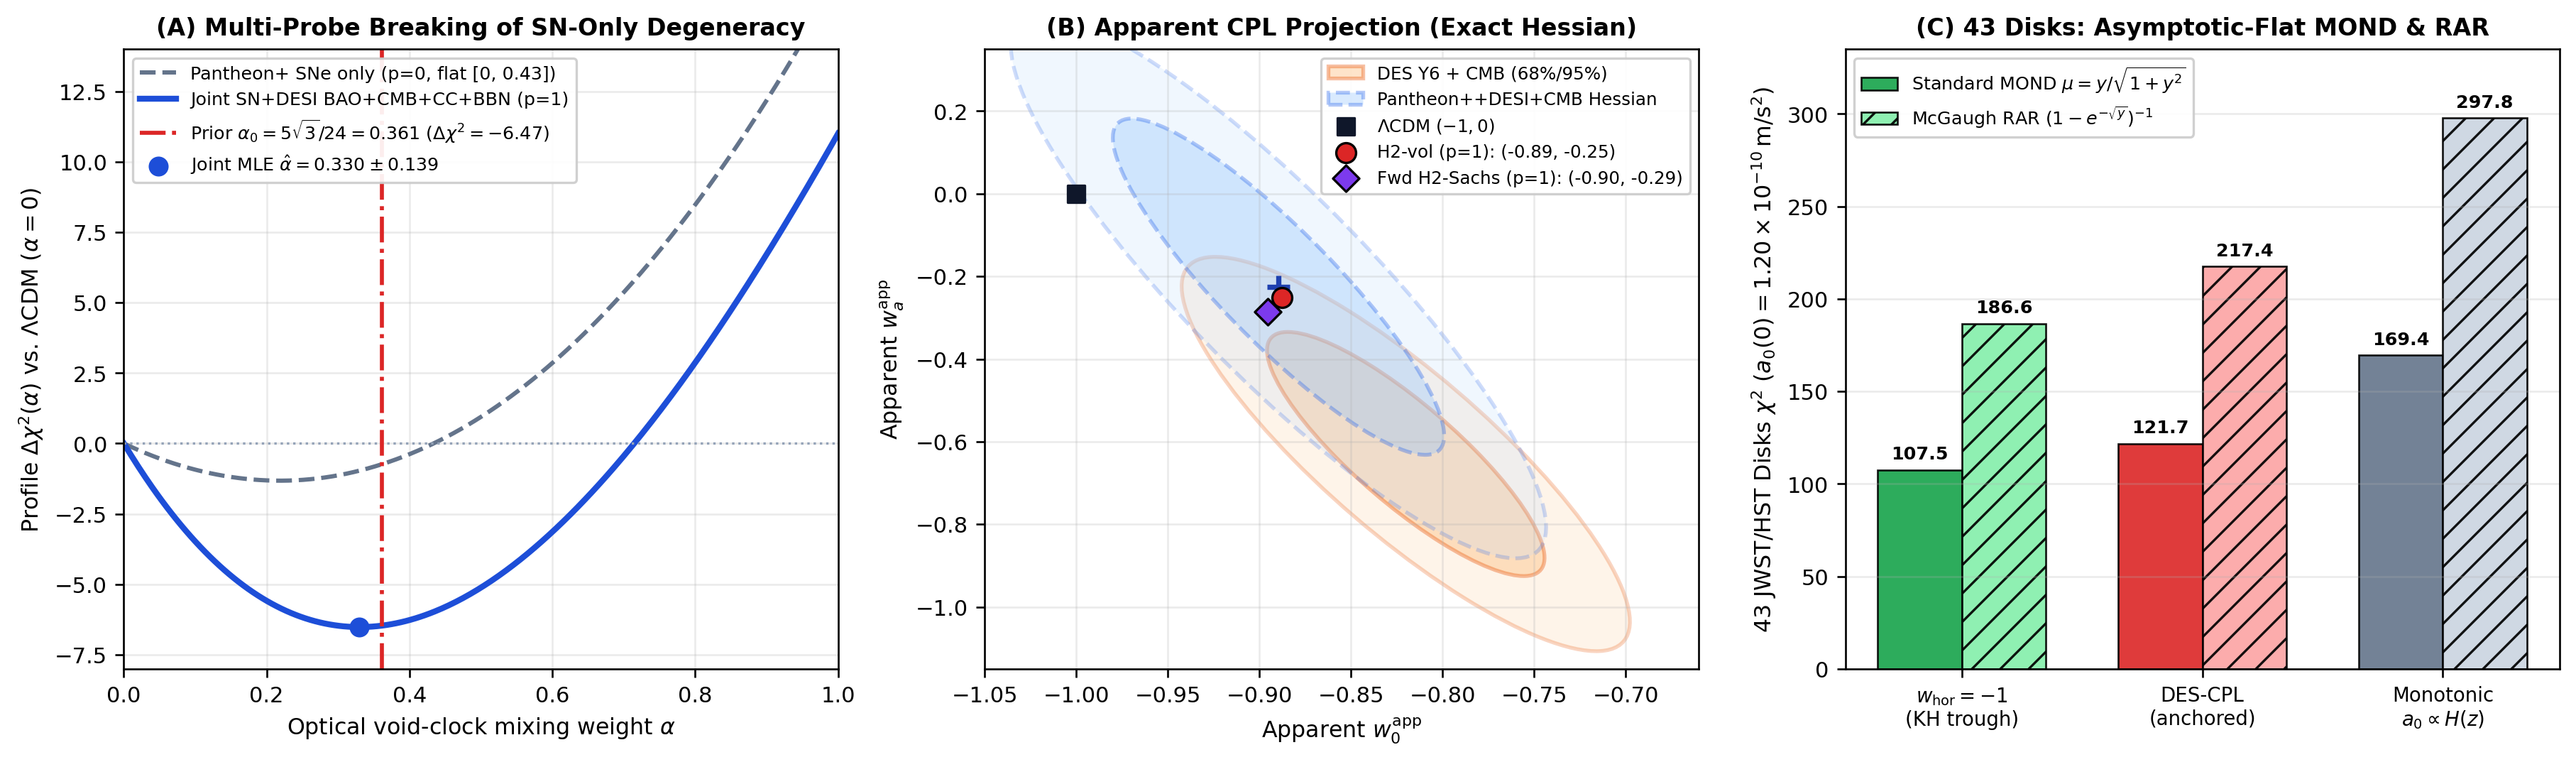
\includegraphics[width=0.99\textwidth]{fig_sub4_void_clock_des2026_and_galactic_dip_en.png}
    \caption{(A) Breaking of the \texttt{Pantheon+}-only $\alpha$--$\Omega_{m,0}$ degeneracy (dashed gray plateau) by direct joint fitting to \texttt{Pantheon++DESI BAO+CMB $\theta_*$+CC+BBN} ($N=1,610$, solid blue, $\hat{\alpha}_{\mathrm{MLE}} = 0.330 \pm 0.139$, $\Delta\chi^2 = -6.52$; prior $\alpha_0 = 0.3608$, $\Delta\chi^2 = -6.47$); (B) illustrative 2D $(w_0^{\mathrm{app}}, w_a^{\mathrm{app}})$ plane using the exact $5\times 5$ Hessian covariance of \texttt{M1b} ($-0.8895 \pm 0.0597, -0.2250 \pm 0.2686, \rho=-0.8860$) and \texttt{DES} Y6 + CMB \cite{DES2026DynDE}; and (C) 43 \texttt{JWST/HST} disk test \cite{ManceraPina2025} using asymptotic-flat Standard MOND \cite{Milgrom1983} and McGaugh RAR \cite{McGaugh2016} kernels.}
    \label{fig:sub4-synthesis}
\end{figure}

\begin{table}[ht!]
\centering
\scriptsize
\setlength{\tabcolsep}{2.6pt}
\renewcommand{\arraystretch}{1.13}
\resizebox{\textwidth}{!}{%
\begin{tabular}{llcccccc}
\toprule
\textbf{Model Variant \& Epistemic Status} & \textbf{$k_{\mathrm{tot}}$ ($k_{\mathrm{dark}}$)} & \textbf{Best $(H_0,\;\Omega_{m,0})$ on $N=1610$} & \textbf{\texttt{Pantheon+} $\chi^2_{\mathrm{SN}}$ ($1580$)$^{\S}$} & \textbf{\texttt{DESI} BAO $\chi^2$ ($13$) / CMB $\chi^2_{\theta_*}$} & \textbf{Joint $N=1610$ $\chi^2$ ($\Delta\chi^2$ vs.\ \texttt{M0})} & \textbf{Joint $N=1610$ $\Delta\mathrm{AIC}$ / $\Delta\mathrm{BIC}$} & \textbf{43 Disks $\chi^2$ (Std.\ MOND / RAR)$^{\dagger}$} \\
\midrule
Standard Flat $\Lambda$CDM (\texttt{M0}, joint baseline) & $4$ ($1$: $\Omega_{c,0}$) & $(68.56,\;0.2963)$ & $1390.57$ ($1387.33$ fix) & $10.73$ / $0.005$ & $1407.67$ ($0.00$) & $0.00$ / $0.00$ & $107.53$ / $186.55$ (KH) \\
Homogeneous CPL (\texttt{M1a}, DES Y6+CMB fixed) & $6$ ($3$: $\Omega_{c,0},w_0,w_a$) & $(67.50,\;0.3097)$ & $1386.97$ ($1387.30$ fix) & $9.83$ / $0.005$ & $1403.42$ ($-4.24$) & $-0.24$ / $+10.52$ & $121.65$ / $217.44$ (anc.) \\
Homogeneous CPL (\texttt{M1b}, free $w_0,w_a$ fit) & $6$ ($3$: $\Omega_{c,0},w_0,w_a$) & $(67.32,\;0.3061)$ & $1386.06$ & $8.68$ / $0.000$ & $1401.14$ ($-6.53$) & $-2.53$ / $+8.24$ & Erases $z=0.6316$ dip \\
Unweighted Pure Timescape ($\alpha=1$, \textbf{H1}) \cite{Wiltshire2009PRD} & $4$ ($1$: $\Omega_{c,0}$) & $(66.42,\;0.3343)$ & $1401.41$ ($1403.83$ fix) & $10.44$ / $0.001$ & $1418.69$ ($+11.02$) & $+11.02$ / $+11.02$ & Not modeled \\
Constant-Weight \textbf{H2a} ($p=0$, $\alpha_0=0.3608$) & $4$ ($1$, phenom.) & $(69.28,\;0.3429)$ & $1389.52$ ($1386.59$ fix) & $16.47$ / $0.043^{\ddagger}$ & $1413.23$ ($\mathbf{+5.56}$) & $+5.56$ / $+5.56$ & \textbf{Ruled out by BAO+CMB} \\
\midrule
\textbf{Void-Volume \texttt{H2-vol} ($p=1$, prior $\alpha_0=0.3608$)} & $4$ ($1$, phenom.) & $(\mathbf{67.52},\;\mathbf{0.3093})$ & $\mathbf{1386.09}$ ($1386.31$ fix) & $\mathbf{8.68}$ / $\mathbf{0.000}$ & $\mathbf{1401.20}$ ($\mathbf{-6.47}$) & $\mathbf{-6.47}$ / $\mathbf{-6.47}$ & $\mathbf{107.53}$ / $\mathbf{186.55}$ (dip) \\
\textbf{Void-Volume \texttt{Forward H2-Sachs} ($p=1$, $\alpha_0$)} & $4$ ($1$, phenom.) & $(\mathbf{67.72},\;\mathbf{0.3062})$ & $\mathbf{1386.04}$ ($1386.11$ fix) & $\mathbf{8.82}$ / $\mathbf{0.000}$ & $\mathbf{1401.30}$ ($\mathbf{-6.37}$) & $\mathbf{-6.37}$ / $\mathbf{-6.37}$ & $\mathbf{107.53}$ / $\mathbf{186.55}$ (dip) \\
\textbf{Void-Volume \texttt{H2-vol} ($p=1$, free $\hat{\alpha}=0.330$)} & $5$ ($2$: $\Omega_{c,0},\alpha$) & $(67.60,\;0.3080)$ & $1386.00$ & $8.76$ / $0.000$ & $1401.15$ ($-6.52$) & $-4.52$ / $+0.87$ & $\mathbf{107.53}$ / $\mathbf{186.55}$ (dip) \\
Sensitivity \texttt{H2-vol} ($p=2$, $\alpha_0=0.3608$) & $4$ ($1$, $\Delta k_{\mathrm{hyp}}=1$) & $(67.57,\;0.3059)$ & $1386.03$ ($1386.16$ fix) & $8.78$ / $0.001$ & $1401.25$ ($-6.42$) & $-4.42$ / $+0.96$ & $\mathbf{107.53}$ / $\mathbf{186.55}$ (dip) \\
\bottomrule
\end{tabular}%
}
\caption{Direct multi-probe likelihood comparison across all $N=1,610$ bundled cosmological data points (\texttt{Pantheon+} $1,580$ + \texttt{DESI} BAO $13$ + Moresco CC $15$ + \texttt{Planck} CMB $100\theta_*$ + Cooke BBN $\omega_b$) and $43$ \texttt{JWST/HST} disks (\texttt{verify\_C9}, \texttt{verify\_C6\_C7}). $^{\S}$Parentheses show fixed-Planck ($\Omega_{m,0}=0.3153$) \texttt{Pantheon+}-only $\chi^2_{\mathrm{SN}}$, where $\Delta\chi^2_{\mathrm{SN}} \in [-1.21,-0.74]$ is statistically equivalent to $\Lambda$CDM ($1387.33$). Without CC ($N=1,595$: \texttt{SN+BAO+CMB+BBN}), \texttt{M0} gives $1401.35$, \textbf{H2-vol} ($p=1$) gives $1394.78$ ($\Delta\chi^2 = \mathbf{-6.57}$), and \textbf{Forward \texttt{H2-Sachs}} ($p=1$) gives $1394.87$ ($\Delta\chi^2 = \mathbf{-6.48}$). $^{\dagger}$Evaluated with asymptotic-flat Standard MOND \cite{Milgrom1983} and McGaugh RAR \cite{McGaugh2016} at $a_0(0)=1.20\times 10^{-10}\;\mathrm{m\,s^{-2}}$ (monotonic $a_0 \propto H(z)$ gives $169.44$ / $297.76$). $^{\ddagger}$At fixed Planck parameters, constant-weight \textbf{H2a} ($p=0$) gives $100\theta_* = 1.0230$ ($\chi^2_{\theta_*} = 3408.5$).}
\label{tab:multiprobe}
\end{table}

\section{Discussion: Multi-Probe Synthesis, Methodological Limits, and \texttt{Euclid} Tests}
\begin{enumerate}
    \item \textbf{Why Direct \texttt{BAO + CMB $\theta_*$} Testing Is Essential:} While \texttt{Pantheon+} alone cannot distinguish $\alpha \in [0, 0.43]$ from $\Lambda$CDM, combining \texttt{Pantheon+} directly with \texttt{DESI} BAO and \texttt{Planck} $\theta_*$ accomplishes two decisive tasks: first, it rules out unphysical $z$-independent void weighting (\textbf{H2a}, $p=0$, $\Delta\chi^2 = +5.56$) because voids vanish prior to structure formation; second, under physical void-volume weighting $\alpha_{\mathrm{eff}}(z) = \alpha f_v(z)/f_{v,0}$ ($p=1$), it resolves the opposite $\Omega_{m,0}$ pulls of SNe~Ia ($\Omega_{m,0} \approx 0.333$) and BAO+CMB ($\Omega_{m,0} \approx 0.296$ in $\Lambda$CDM), yielding $\hat{\alpha}_{\mathrm{MLE}} = 0.330 \pm 0.139$ ($\Delta\chi^2 = -6.52$, $\sim 2.55\sigma$). We emphasize that $\Delta\chi^2 \approx -6.5$ represents moderate multi-probe preference (matching 6-parameter free CPL \texttt{M1b} with two fewer parameters, $\Delta\mathrm{BIC} = -14.71$) rather than a $5\sigma$ exclusion of $\Lambda$CDM, and reconciles \texttt{Pantheon++DESI+CMB} with Efstathiou's \cite{Efstathiou2025SN} $\sim 0.04\;\mathrm{mag}$ \texttt{DES-SN5YR} offset audit.
    \item \textbf{Methodological Scope and Open Frontiers:} (i) Pure Timescape achieves stronger fits when light-curve nuisance parameters ($\alpha x_1, \beta c$) are re-fitted from raw photometry \cite{LaneWiltshire2025MNRAS,SeifertWiltshire2025MNRAS} rather than standard SALT2 \texttt{Pantheon+} covariances; (ii) the 43 \texttt{JWST/HST} disks ($0.787 \le z \le 1.03$) probe the post-trough $z \approx 0.9$ amplitude of $a_0(z)$, so directly bracketing $z_{\mathrm{dip}} = 0.6316$ awaits dense $0.3 \le z \le 0.8$ IFU surveys; and (iii) \textbf{H1} and \textbf{H2-vol} / \textbf{Forward \texttt{H2-Sachs}} remain phenomenological effective models awaiting a single inhomogeneous 4D metric derivation.
    \item \textbf{Falsification in \texttt{Euclid} + \texttt{Rubin LSST}:} Splitting SNe~Ia by sightline void fraction must show $w_0^{\mathrm{app}} \to -0.89$ along void-rich sightlines vs.\ $-1.00$ along filament-rich sightlines, while tomographic rotation curves test $a_0(z)/[cH(z)|1-q(z)|] = \mathrm{const}$.
\end{enumerate}

\paragraph{Data and Code Availability.} All four standalone scripts (\texttt{verify\_C9}, \texttt{verify\_C5}, \texttt{verify\_C3\_C4}, \texttt{verify\_C6\_C7}; executable with \texttt{NumPy}/\texttt{SciPy} alone in $\sim 10\;\mathrm{s}$) and all nine raw observational datasets are bundled in \texttt{supplementary\_code\_and\_data/}.

\begin{thebibliography}{99}
\bibitem{DES2026DynDE} DES Collaboration, \textit{Constraints on Dynamical Dark Energy from Multiple Probes in the Full Dark Energy Survey}, arXiv:2605.27221 (2026).
\bibitem{DESSN5YR2024} DES Collaboration, \textit{The Dark Energy Survey: Cosmology Results with $\sim 1500$ New High-redshift Type Ia Supernovae Using the Full 5 Year Dataset}, Astrophys.\ J.\ Lett.\ \textbf{973}, L14 (2024), arXiv:2401.02929.
\bibitem{DESIDR2_2025} DESI Collaboration, \textit{DESI DR2 Results II: Measurements of Baryon Acoustic Oscillations and Cosmological Constraints}, arXiv:2503.14738 (2025).
\bibitem{Efstathiou2025SN} G.~Efstathiou, \textit{Evolving Dark Energy or Supernovae Systematics?}, Mon.\ Not.\ R.\ Astron.\ Soc.\ \textbf{538}, 875 (2025), arXiv:2408.07175.
\bibitem{Brout2022} D.~Brout \textit{et al.}, \textit{The Pantheon+ Analysis: Cosmological Constraints}, Astrophys.\ J.\ \textbf{938}, 110 (2022), arXiv:2202.04077.
\bibitem{LaneWiltshire2025MNRAS} Z.~G.~Lane, A.~Seifert, R.~Ridden-Harper, and D.~L.~Wiltshire, \textit{Cosmological foundations revisited with Pantheon+}, Mon.\ Not.\ R.\ Astron.\ Soc.\ \textbf{536}, 1752 (2025), arXiv:2311.01438.
\bibitem{SeifertWiltshire2025MNRAS} A.~Seifert, Z.~G.~Lane, M.~Galoppo, R.~Ridden-Harper, and D.~L.~Wiltshire, \textit{Supernovae evidence for foundational change to cosmological models}, Mon.\ Not.\ R.\ Astron.\ Soc.\ Lett.\ \textbf{537}, L55 (2025), arXiv:2412.15143.
\bibitem{Wiltshire2009PRD} D.~L.~Wiltshire, \textit{Average observational quantities in the timescape cosmology}, Phys.\ Rev.\ D \textbf{80}, 123512 (2009), arXiv:0909.0749.
\bibitem{Milgrom1983} M.~Milgrom, \textit{A modification of the Newtonian dynamics as a possible alternative to the hidden mass hypothesis}, Astrophys.\ J.\ \textbf{270}, 365 (1983).
\bibitem{McGaugh2016} S.~S.~McGaugh, F.~Lelli, and J.~M.~Schombert, \textit{Radial Acceleration Relation in Rotationally Supported Galaxies}, Phys.\ Rev.\ Lett.\ \textbf{117}, 201101 (2016), arXiv:1609.05917.
\bibitem{ManceraPina2025} P.~E.~Mancera Pi\~na, E.~M.~Di~Teodoro, S.~M.~Fall, A.~Marasco, M.~Kriek, and M.~Martorano, \textit{Kinematic scaling relations of disc galaxies from ionised gas at $z \sim 1$ and their connection with dark matter haloes}, Astron.\ Astrophys.\ (2025), arXiv:2511.08685.
\bibitem{Kantowski1969} R.~Kantowski, \textit{Corrections in the Luminosity-Redshift Relations of the Homogeneous Friedmann Models}, Astrophys.\ J.\ \textbf{155}, 89 (1969).
\bibitem{DyerRoeder1973} C.~C.~Dyer and R.~C.~Roeder, \textit{Distance-Redshift Relations for Universes with Some Intergalactic Medium}, Astrophys.\ J.\ Lett.\ \textbf{180}, L31 (1973); Astrophys.\ J.\ \textbf{174}, L115 (1972).
\bibitem{Weinberg1976} S.~Weinberg, \textit{Apparent Luminosities in a Locally Inhomogeneous Universe}, Astrophys.\ J.\ Lett.\ \textbf{208}, L1 (1976).
\bibitem{Planck2018VI} N.~Aghanim \textit{et al.} (Planck Collaboration), \textit{Planck 2018 results. VI. Cosmological parameters}, Astron.\ Astrophys.\ \textbf{641}, A6 (2020).
\bibitem{TauCoreZenodo2026} J.~Olcsak, \textit{Covariant Horizon-Coupled Modified Gravity and Multi-Probe Verification Suite}, Zenodo (2026), \href{https://doi.org/10.5281/zenodo.24305895}{doi:10.5281/zenodo.24305895} and \href{https://doi.org/10.5281/zenodo.24354218}{doi:10.5281/zenodo.24354218}.
\end{thebibliography}

\end{document}
